\documentclass[onecolumn, draftclsnofoot,10pt, compsoc]{IEEEtran}
\usepackage{graphicx}
\usepackage{url}
\usepackage{setspace}

\usepackage{geometry}
\geometry{textheight=9.5in, textwidth=7in}

\usepackage{listings}
\usepackage{color}

\definecolor{dkgreen}{rgb}{0,0.6,0}
\definecolor{gray}{rgb}{0.5,0.5,0.5}
\definecolor{mauve}{rgb}{0.58,0,0.82}

\lstdefinestyle{php}
{
   frame=tb,
   language=PHP,
   aboveskip=3mm,
   belowskip=3mm,
   showstringspaces=false,
   columns=flexible,
   basicstyle={\small\ttfamily},
   numbers=none,
   numberstyle=\tiny\color{gray},
   keywordstyle=\color{blue},
   commentstyle=\color{dkgreen},
   stringstyle=\color{mauve},
   breaklines=true,
   breakatwhitespace=true,
   tabsize=3
}

\lstdefinestyle{javascript}
{
   frame=tb,
   language=C++,
   aboveskip=3mm,
   belowskip=3mm,
   showstringspaces=false,
   columns=flexible,
   basicstyle={\small\ttfamily},
   numbers=none,
   numberstyle=\tiny\color{gray},
   keywordstyle=\color{blue},
   commentstyle=\color{dkgreen},
   stringstyle=\color{mauve},
   breaklines=true,
   breakatwhitespace=true,
   tabsize=3
}

\lstdefinestyle{java}
{
   frame=tb,
   language=Java,
   aboveskip=3mm,
   belowskip=3mm,
   showstringspaces=false,
   columns=flexible,
   basicstyle={\small\ttfamily},
   numbers=none,
   numberstyle=\tiny\color{gray},
   keywordstyle=\color{blue},
   commentstyle=\color{dkgreen},
   stringstyle=\color{mauve},
   breaklines=true,
   breakatwhitespace=true,
   tabsize=3
}

% 1. Fill in these details
\def \CapstoneTeamName{		The Cleverly Named Team}
\def \CapstoneTeamNumber{		14}
\def \GroupMemberOne{			Omeed Habibelahian}
\def \GroupMemberTwo{			Bradley Imai}
\def \GroupMemberThree{			Dylan Tomlinson}
\def \CapstoneProjectName{		"I Heart Corvallis" Mobile Application}
\def \CapstoneSponsorCompany{	Corvallis Community Relations Office}
\def \CapstoneSponsorPerson{		Lyndi-Rae Petty}

% 2. Uncomment the appropriate line below so that the document type works
\def \DocType{		%Problem Statement
				%Requirements Document
				%Technology Review
				%Design Document
				%Progress Report
        Final Report
				}

\newcommand{\NameSigPair}[1]{\par
\makebox[2.75in][r]{#1} \hfil 	\makebox[3.25in]{\makebox[2.25in]{\hrulefill} \hfill		\makebox[.75in]{\hrulefill}}
\par\vspace{-12pt} \textit{\tiny\noindent
\makebox[2.75in]{} \hfil		\makebox[3.25in]{\makebox[2.25in][r]{Signature} \hfill	\makebox[.75in][r]{Date}}}}
% 3. If the document is not to be signed, uncomment the RENEWcommand below
\renewcommand{\NameSigPair}[1]{#1}

%%%%%%%%%%%%%%%%%%%%%%%%%%%%%%%%%%%%%%%
\begin{document}
\begin{titlepage}
    \pagenumbering{gobble}
    \begin{singlespace}
    	
\includegraphics[height=4cm]{coe_v_spot1}
        \hfill
        % 4. If you have a logo, use this includegraphics command to put it on the coversheet.
        %\includegraphics[height=4cm]{CompanyLogo}
        \par\vspace{.2in}
        \centering
        \scshape{
            \huge CS Capstone \DocType \par
            {\large\today}\par
            \vspace{.5in}
            \textbf{\Huge\CapstoneProjectName}\par
            \vfill
            {\large Prepared for}\par
            \Huge \CapstoneSponsorCompany\par
            \vspace{5pt}
            {\Large\NameSigPair{\CapstoneSponsorPerson}\par}
            {\large Prepared by }\par
            Group\CapstoneTeamNumber\par
            % 5. comment out the line below this one if you do not wish to name your team
            %\CapstoneTeamName\par
            \vspace{5pt}
            {\Large
                \NameSigPair{\GroupMemberOne}\par
                \NameSigPair{\GroupMemberTwo}\par
                \NameSigPair{\GroupMemberThree}\par
            }
            \vspace{20pt}
        }
        \begin{abstract}
        % 6. Fill in your abstract
        		This document acts as the complete notebook for the I Heart Corvallis mobile application project. It details the project requirements and design, technology reviews for various aspects of the project, and our team's weekly blog posts detailing our progress. It also includes documentation on how the project works and how to install and run the application, and it provides some functionality flowcharts. The team also provides conclusions and reflections on the past year, and the appendices provide notable code listings and screenshots from the project.
        \end{abstract}
    \end{singlespace}
\end{titlepage}
\newpage
\pagenumbering{arabic}
\tableofcontents
% 7. uncomment this (if applicable). Consider adding a page break.
%\listoffigures
%\listoftables
\clearpage

% 8. now you write!
\section{Introduction}
  The "I Heart Corvallis" mobile application was conceptualized by the Corvallis Community Relations office to complement their larger "I Heart Corvallis" initiative. The CCR office noticed that many OSU students do not engage much with the greater community and prefer to interact with the OSU community itself, so they started this initiative to build and promote a strong and cooperative relationship between the OSU community and the greater Corvallis community. The goal of the mobile app is to inform students about the various community events, activities, and service opportunities available to them around the community, as well as to give them an incentive to engage in these activities.
  Our client was Lyndi-Rae Petty, the Graduate Teaching Assistant at the Corvallis Community Relations office, a subset of the Office of Student Life. The development team consisted of Omeed Habibelahian, Bradley Imai, and Dylan Tomlinson. All three of us were heavily involved in nearly all aspects of the application, and we often helped each other out when one of us was stuck on a particular section of the development. It was not so much that one of us took a particular role; we were all involved in the various aspects of development and implementation, as well as in communicating updates and changes with our client. There were, however, a few aspects of the development that we each took more control of. Omeed handled more of the implementation of the administrative website, Dylan was in charge of user security on both the mobile application and the administrative website, and Bradley put in quite a bit of work on the design of the user interface of the mobile application.
  Our client primarily took the role of supervisor of the project. Every week we would meet with her to discuss the changes we made and new features we implemented, as well as what we had to do next, and she gave input on how she felt about our changes and anything she wanted done differently. When we needed to reach out to another organization or source for guidance or help, we would describe our situation to her, and she would take charge of reaching out to these organizations.
  \newpage

\section{Requirements Document}
  [page placeholder]\newpage
  [page placeholder]\newpage
  [page placeholder]\newpage
  [page placeholder]\newpage
  [page placeholder]\newpage
  [page placeholder]\newpage
  [page placeholder]\newpage
  [page placeholder]\newpage
  \subsection{Requirement Modifications}
    The two requirements that were changed were the implementation of the ONID login and the database usage. \\ \\
    We did not implement the ONID login system, or CAS, into the application, as we were unable to figure out how to implement CAS on a mobile device. The documentation for integrating CAS into a website is fairly straightforward, but this documentation does not translate to mobile applications the same way. We did reach out to some other resources within OSU, like Derek Whiteside (Director of Web and Mobile Services) and Andrew Morgan (Systems Administrator for Identity and Access Management), and we received some valuable information from the latter source, but we were nonetheless unable to complete the requirement. We made sure our client was aware of this, and she gave us the green light to proceed without implementing CAS. Instead, we implemented a universal login system that asks the user if they are a student/faculty member during the signup process. \\ \\
    We also did not use two databases for the project, as mentioned in the document. We are not exactly sure what our reasoning was behind that idea. It is possible that we meant two tables rather than two databases, but we ended up only needing one table for all of the tables for the application and administrative website. Our MySQL database consisted of 11 tables. \\ \\
  \subsection{Updated Gantt Chart}
    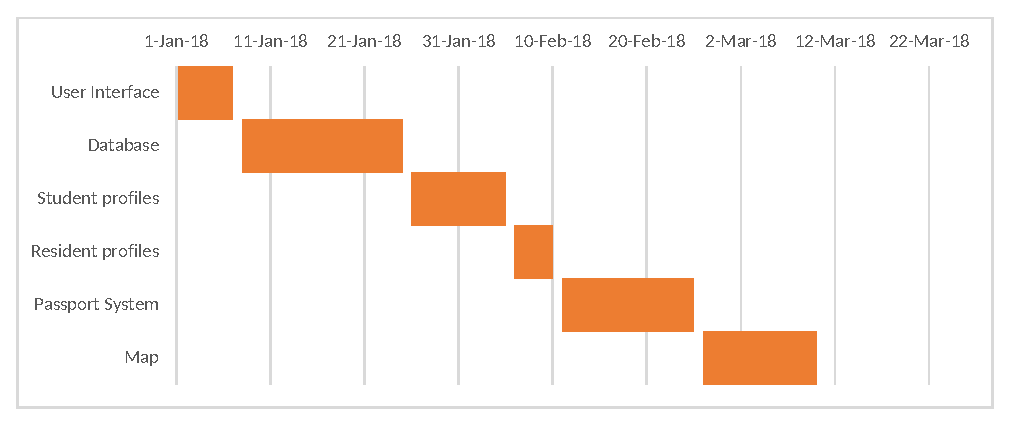
\includegraphics[height=7cm]{ganttchart}
  \newpage

\section{Design Document}
  [page placeholder]\newpage
  [page placeholder]\newpage
  [page placeholder]\newpage
  [page placeholder]\newpage
  [page placeholder]\newpage
  [page placeholder]\newpage
  [page placeholder]\newpage
  [page placeholder]\newpage
  [page placeholder]\newpage
  [page placeholder]\newpage
  [page placeholder]\newpage
  [page placeholder]\newpage
  \subsection{Design Modifications}
    There were a few design aspects that we changed or removed altogether. \\ \\
    The plan to integrate a social media API, such as Instagram, was scrapped, as it did not fit into the user interface of our application and was deemed unnecessary. The plan for an in-app administrative interface was also changed to a web-based interface. This change was requested by our client, who told us that it would be easier for her to maintain the content of the application on her computer rather than on her phone in the application. \\ \\
    We changed the application from an HTML-based application to a stock Android, Java-based application. As a result of this, we also strayed away from using Semantic UI in the application. We made this change because in order to enable PHP on the application, we had to install PHP onto the device, which we were having trouble implementing. Android also has significantly more documentation for these languages, which helped us out quite a bit in the long run. \\ \\
    We did not focus on scaling the UI of the application. This design decision fell out of our scope as we focused on the main UI and functionality of the app. Our client was satisfied with the condition of the application, prompting us to consider our development of our application finished in early May.
  \newpage

\section{Tech Review}
  [page placeholder]\newpage
  [page placeholder]\newpage
  [page placeholder]\newpage
  [page placeholder]\newpage
  [page placeholder]\newpage
  [page placeholder]\newpage
  [page placeholder]\newpage
  [page placeholder]\newpage
  [page placeholder]\newpage
  [page placeholder]\newpage
  [page placeholder]\newpage
  [page placeholder]\newpage
  [page placeholder]\newpage
  [page placeholder]\newpage
  [page placeholder]\newpage
  [page placeholder]\newpage
  [page placeholder]\newpage
  [page placeholder]\newpage
  [page placeholder]\newpage
  [page placeholder]\newpage
  [page placeholder]\newpage
  [page placeholder]\newpage
  [page placeholder]\newpage
  [page placeholder]\newpage

\section{Weekly Blog Posts}
  \subsection{Omeed}
    \subsubsection{Fall 2017}
      \paragraph{Week 1}
      This week I thought about which projects I wanted to work on, and I submitted my project preferences. I also spoke with Bradley about working on the I Heart Corvallis mobile app project, contacted Lyndi-Rae Elisabeth Petty (the project's client), and got approved to work on that project. \\ \\

      \paragraph{Week 2}
      This week we were officially assigned to our project groups. Brad emailed our client our contact information and asked for good meeting times for next week. When she responded with potential meeting times for next week, I initiated discussion with my groupmates to figure out when would be the best time to meet with her, and when we figured out the best time, Brad let our client know, and she confirmed that time with us. I also met with the full group for the first time after class on Thursday. \\ \\
      Next week we will meet with our client planned for next Wednesday (October 11) at 2pm to have a deeper discussion about what the project entails. \\ \\

      \paragraph{Week 3}
      This week I wrote the rough draft of the problem statement for my project. At that point, we hadn't met with our clients yet so I wasn't really able to base much of the rough draft on the client's explanation of the project. Now that we've met with our clients, we'll be able to write a more complete and thorough final draft of the problem statement. \\ \\
      On Wednesday we met with our clients for the first time. They told us their vision for the app and their timeline for completing various aspects of the app, and we had a conversation about the app's design and features, as well as some of what we'll need from them. Hopefully soon they'll nail down exactly what they want in the app so we can put these specifications in our design document. \\ \\
      We met with our TA for the first time this week, and we're going to meet with him at the same time (Wednesdays at 3:20pm) every week this term. \\ \\
      I also started making some drawings of what the app's pages could look like. Next week I'm going to share my drawings with the rest of the team, and they'll share any drawings they make as well. \\ \\
      I also found some good software that could help make it easier to implement the app for both Android and iOS. Since not all languages work well on both Android and iOS, it's important that we're able to find a way to implement the app in such a way that we don't have to implement it completely differently (such as in a completely different language) for Android than for iOS. I found Xamarin (which is in Visual Studio) and it will allow for cross-platform app implementation in C\#. I'll continue to look into the best options for easy cross-platform development, since coding in different languages for Android and iOS would significantly increase the amount of time it takes to complete this project. \\ \\

      \paragraph{Week 4}
      This week we focused on completing and turning in our Problem Statement. On Monday the three of us got together at the library to write the final draft of the Problem Statement. We got most of it finished on Monday, and on Tuesday we went to Kirsten's office hours and the Writing and Research Center to receive feedback on our writing. I posted our final draft to OneNote and emailed Lyndi our completed final draft on Thursday. Kirsten gave us more feedback on OneNote, and Brad and I got together to figure out how to take her of her recommended fixes. I completed the fixes and reposted the final draft on OneNote and re-emailed it to Lyndi early Friday morning. \\ \\
      Next week we plan to write the rough draft of the requirements document, and we will meet with Lyndi and Jon (our clients) again soon to continue talks on the application. \\ \\

      \paragraph{Week 5}
      This week we scheduled another meeting with Lyndi to discuss the next steps for the planning of the project. We now have a tentative meeting time with her each week (Wednesdays at 2pm). I showed her the Photoshop app mockups I made of the initial login screen and the homepage, and we told her we can come up with more designs for the app so she can get an idea of what the final version of the app could look like. We also informed her that depending on whether we take the route of implementing the app in a cross-platform fashion or we take the route of building the Android app in Android Studio and the iOS app in Xcode, we could potentially run into a time constraint, as the latter option would essentially require us to make two separate apps, since we would finish the Android app first and then the iOS app. She emailed us some resources to help us figure out what would be the best option, but she was receptive to and accepting of the fact that we may potentially not have enough time to code both versions of the app. \\ \\
      We also wrote the rough draft of our Requirements Document this week. We began compiling information for the document on Thursday, and we met in the library Friday afternoon to continue working on the rough draft. I finished the rough draft Friday night. We plan to use the feedback we receive to make a more complete Requirements Document for next week. \\ \\

      \paragraph{Week 6}
      This week I met with Lyndi along with the rest of our group. We have pretty much nailed down a weekly meeting time of Wednesdays at 2pm. We discussed the focus group that was happening later that day, as well as more app design concepts, the requirements document, and cross-platform implementation and keeping the iOS version of the app a stretch goal. We also met with our TA. We recorded a lot of useful information based on the discussions that occurred in the focus group that day. \\ \\
      I also worked with the other team members to complete the final draft of the requirements document and send it to Lyndi. She emailed back with a couple of small corrections, and I made those corrections and resent it to her. She emailed Kevin and Kirsten on Friday letting them know that she received and approved the final draft of the requirements document. \\ \\
      Next week I will work on completing the rough draft of the technology review document, and next Wednesday (11/8) our group will discuss the focus group discussion that occurred this past Wednesday. \\ \\

      \paragraph{Week 7}
      This week we met with Lyndi on Wednesday to reflect on last week's focus group and the feedback we were given by the focus group attendees. There's another focus group scheduled for next Tuesday, and we'll use the information we've compiled from both focus group sessions to make more concrete decisions on what we're going to include in the app. We've been able to nail down much of what the app will entail already, though. We also met with our TA on Wednesday. That same day I created a Google Doc with a table that we will fill with topics for the Tech Review document and decide who will cover each topic. We were originally planning to meet this week to fill out the table and figure out who will cover what topics, but that has been pushed back to this weekend. \\ \\
      This weekend and next week we will write our Tech Review rough draft and take a look at what feedback we receive at the second focus group session that's scheduled for Tuesday. \\ \\

      \paragraph{Week 8}
      This week was a pretty light week for our group. I completed the rough draft of my Tech Review document on Tuesday. Our client held another focus group for the I Heart Corvallis initiative on Tuesday. We didn’t meet with her this week, as there wasn’t a lot of new things to discuss this week, but during our next meeting with her, we will go overview the feedback given in this week’s focus group. We also met with our TA this week. This weekend and next week I will complete my final draft of the Tech Review document and work on the rough draft of the Design Document so I can receive feedback on it. Our next meeting time with both our client and our TA are not completely determined yet, either, as Thanksgiving is next week. We will communicate with both our client and our TA to figure out what the plan is for next week. \\ \\

      \paragraph{Week 9}
      This week was a short and light one. I completed the final draft of my Tech Review document on Tuesday. On Thursday, I made a Google Doc for the team containing the template for the Design Document. We will work on the Design Document next week. We also plan to meet with Lyndi next week to get back up to speed (since we haven't met since November 8) and discuss the feedback she received at the last focus group. \\ \\

      \paragraph{Week 10}
      This week we completed the final draft of the Design Document. I went to Kirsten's office hours twice with Bradley to get some more clarification on the composition of the Design Document. Once we completed the final draft, I emailed it to Lyndi so she could give us any feedback she had and approve it if it looked good. She approved the final draft and emailed Kevin and Kirsten letting them know she had received and approved it. I've already started the Fall Term Progress Report, and next week will complete it and make the corresponding presentation. Over Winter Break, we plan to begin implementation of the application. \\ \\

    \subsubsection{Winter 2018}
      \paragraph{Week 1}
      Over Winter Break we got a lot of the basic app layout and page creation completed, and we started implementing various layouts and attributes to each page. We met with Lyndi this week to discuss our progress on the app, what both our and their timelines look like for this term and next term, and what we're currently working on with the app. We also set up weekly group work times so we can have set times dedicated to working on the app as a group. Next week we will continue working on creating our MySQL databases and connecting the app to the databases, as well as implementing more layouts and attributes to the various pages of the app. \\ \\

      \paragraph{Week 2}
      Over Winter Break we got a lot of the basic app layout and page creation completed, and we started implementing various layouts and attributes to each page. We met with Lyndi this week to discuss our progress on the app, what both our and their timelines look like for this term and next term, and what we're currently working on with the app. We also set up weekly group work times so we can have set times dedicated to working on the app as a group. Next week we will continue working on creating our MySQL databases and connecting the app to the databases, as well as implementing more layouts and attributes to the various pages of the app. \\ \\

      \paragraph{Week 3}
      This week was a very productive week for us. After working for quite a bit of time to connect the app to our database, on Wednesday I finally got the app connected to my PHP scripts that communicate with the database. Once I got that working for our non-student login page, I connected it to our signup page, as well as other pages that will be behind the authentication wall, such as the events page, leaderboard, and resource map. We met with Lyndi on Thursday to show the progress we've made in the past week, and during this meeting we all went to meet with Derek Whiteside of Web and Mobile Services to discuss storage location options for our database, as well as other important mobile application topics, such as security, app branding, CAS (the ONID login), and app lifecycle/maintenance. Next week we will continue integrating our app with our database, and we will begin work on our administrative interface, which Lyndi told us yesterday she would prefer to be in the form of a website rather than an in-app interface. \\ \\

      \paragraph{Week 4}
      This week was a bit lighter of a work week, as we had a lot of work in other classes to do this week. We mostly worked on implementing the administrative interface, which our client told us last week she wanted to be in the form of a website instead of an in-app interface. Bradley initialized the website, while I worked on styling it and furthering its functionality. I integrated Semantic UI to the site, which made it more visually pleasing. I also added some more specific columns to our event database, such as address, latitude, and longitude. We also went through the details of our project to determine what we’ve completed so far and what we have left to do, and we divided up the remaining pieces among the three of us. Next week we will start to work more heavily on our respective pieces of the projects so we can have a Beta version of the app ready by the end of the term. \\ \\

      \paragraph{Week 5}
      This week was a light work week for me as I had midterms in other classes on Wednesday and Friday this week. Nonetheless, I did put in some work on the administrative website. I got most of the Manage Events page working, and I created a home page (index.html) that has quick links to a bunch of other admin pages. We also had our weekly client meeting with Lyndi to discuss our progress the past week and next steps for the project. Dylan got the user session implemented so that the app remembers who's logged in, even when the app is closed. This weekend and next week we plan to create a draft of our Expo poster, as well as create and submit our midterm progress report and presentation. I will also be able to pick up the pace on my share of the work next week as I've now gotten both midterms out of the way. \\ \\

      \paragraph{Week 6}
      This week we got a lot of work done on our app and website, and we also put a decent amount of time aside to work on the midterm progress report and presentation, as well as the draft of our Expo poster. We recorded our presentation and worked on the Expo poster draft on Sunday, and I put together the pieces and finished the video the same day. This week I also set up the event maps, set up the event management webpage, and set up the prize addition and management webpages for our administrative website. We finished the Expo poster draft on Wednesday, and Dylan submitted it the same day. We completed and submitted the midterm progress report Friday afternoon. Now that all of our midterms are out of the way (Brad and Dylan both had midterms this week), next week we're going to focus on working towards finishing the website, as well as implementing geolocation services and the event PIN verification page. We're also going to have to start looking at options for third-party database services to store our data tables long-term. \\ \\

      \paragraph{Week 7}
      This week we got some important parts of the application implemented. Dylan set up password hashing so that account passwords aren't stored as plaintext in the database, but are rather hashed using the PBKDF2 hashing algorithm. He also started implementing PHP prepared statements into our PHP scripts to protect them from MySQL injections. Brad got geolocation services set up for the event map. I replaced AsyncTasks in several activities to AsyncTaskLoaders (and put these loaders in their own pages instead of leaving them as anonymous classes in the activity). This will allow for both less resources being used when performing activity tasks and caching of retrieved data, both of which increase app efficiency. Our main problem this week was that our client recently found out that her position will not be retained after this school year, so we'll need to figure out if that will have any implications for our project. We will look into that situation more next week. Next week we plan to implement features such as geofencing, more AsyncTaskLoaders for activities, updating the completed events database upon entering the correct PIN for an event, and implementing more pages for the administrative website. \\ \\

      \paragraph{Week 8}
      This week we focused on fixing our PHP prepared statements, implementing more AsyncTaskLoaders (to replace AsyncTasks) for our various app pages, and adding the ability for our client to add and manage resource page information and resource map markers. On Wednesday, I implemented the AsyncTaskLoaders, and on Thursday I implemented the resource management pages on the administrative website. We've been fairly consistently looking at our PHP prepared statements, since they'll be important in preventing hackers from messing with our database. However, most of them are not yet working properly, so we're still looking into what's wrong with them and how to fix those statements. We'll continue examining those errors next week. This week we also found out that our project is not in jeopardy despite the uncertain status of our client's position for next year, which is definitely a good sign. Next week we'll continue working on our administrative website and add some of the final remaining pieces into our application. \\ \\

      \paragraph{Week 9}
      This week was a critical week in the progress of our project. We now have a near-complete website, including the ability to log in and out of the site and putting the webpages behind a login wall so users have to log in before accessing any of the webpages. This allows our client to control who can edit in-app content, as they'll be able to authenticate new administrative users after logging into the website themselves. I also enhanced the resource map this week, as the legend is now collapsible and the user can now restrict the map to only show a specific type of resource. I also initialized my final progress report for this term. \\ \\
      One important bug that I ran into on Thursday is that the user's information is not always passed between pages, and the app crashes when trying to log the user's ID as a result. It's not a consistent issue, and it only happens sometimes after officially completing an event and returning to the Dashboard. We'll be looking into that error and figuring out what's causing it in the near future, as it will likely become an annoying issue for the user if it's not resolved. \\ \\

      \paragraph{Week 10}
      This week was largely spent on refining various aspects of the app and patching bugs. On Sunday we set up geofencing for event attendance verification. Now, when a user wants to check into an event, they can only so if they are within range of the event (within 0.1 miles). On Tuesday, I patched a bug where user information wouldn't always get passed around the app and the app would crash when trying to access user information. On Wednesday I added an end date/time for each event and reflected this change on both the website and in the application. And on Thursday I corrected the hex color code for the official Beaver Orange color in our app. We also recorded our final progress report presentation for the term on Thursday. Over the weekend and into next week I'll write my final progress report for the term and prepare the presentation video. We're also meeting (along with our client) with the systems administrator of Identity \& Access Management at OSU to discuss integrated CAS and Single Sign On into our application for the student log-in. \\ \\

    \subsubsection{Spring 2018}
      \paragraph{Week 1}
      This week we got a lot of smaller miscellaneous things done. We set up weekly meeting times with Lyndi (our client) and emailed Andrew (our TA) to schedule weekly TA meetings. I created the survey over Spring Break, and got it fully connected to our app and database throughout the week. On Wednesday I changed the "age" column of the user database to "birthdate" and made it a datetime column to better handle user ages, and I added a date picker for the birthdate to the Settings page. This week I also started editing the app's style to fit OSU branding guidelines. I added branding-approved colors, fonts, icons, and a background image. On Wednesday Dylan introduced the idea of changing the format of the survey response table to allow for the ability to change the number of survey questions, and I recreated that table and restructured the survey response loader and corresponding PHP script to reflect this change. Dylan found a signup bug that caused the signup PHP script to not work and a FileNotFoundException to be thrown, meaning new accounts could not be created. On Friday, Dylan and I successfully fixed this bug, and users can once again sign up for the app. Next week we plan to begin implementation of the CAS login to allow students to sign up and log in with their ONID accounts. We will also continue fixing bugs that we find. \\ \\

      \paragraph{Week 2}
      Due to grad school visits and planning, this week was a lighter week for me. However, Brad and Dylan did a good job of helping out with implementation this week. I've been working on enhancing the student survey to get more information from the user upon signup, such as grade, birth date, and user type (domestic student, international student, resident, visitor, etc.). I also re-added the birthdate preference to the Settings fragment for all users (I had previously made it only shown for non-student users, such as residents or visitors). \\ \\
      We also began implementing the CAS login system for OSU students. We ran into some issues where we would get a Stale Request when trying to use the ONID login, and we're stuck on how to get the user's data back down to the application after validating their ticket. We had our client email Derek Whiteside at Web Services for help directing us to someone who could help with that. Next week we'll continue implementing the CAS login, and I'll continue updating the survey. We'll begin working on adding the ability to add custom images for events soon as well. \\ \\

      \paragraph{Week 3}
      This week was a big week for us. We finally got image upload working for events and resources, so now newly added events and resources can have custom images associated with them. I also implemented the ability for the user to choose, take, and change a profile picture for their account. The profile picture is unique to the device the app is installed on, as it's stored in a local database on the device. I also added indicators for faculty users of the app. This addition can be seen in the page where we ask the user for more basic information, as well as in the Settings page, where you can change your grade and user type preference among other account attributes. I also implemented prepared statements for nearly every PHP script for the app and website. This will really help secure our tables against PHP injection attacks. \\ \\
      We reached out to Derek Whiteside at Web Services, since we’ve ran into a wall integrating CAS login for OSU students and faculty. He has not responded since our client emailed him, and we're beginning to run out of time to implement the feature, so we may ditch CAS integration in favor of one universal login system. Our client is okay with us doing this if we cannot get CAS integrated. \\ \\
      Next week we will patch a couple of remaining bugs and move on to building the demo version of our app, since we will not have reliable Internet access at the Engineering Expo. \\ \\

      \paragraph{Week 4}
      This week we focused on patching some final bugs and implementing the remaining features of the app and website. I fixed the form validation bug on the website and implemented more prepared statements in the PHP scripts. On Wednesday I got the app permissions working, so the app now asks the user for permission to use location services, the camera, and the photo gallery on the device. The former permission is for the event map and event check-in, while the latter two permissions are for the profile picture. \\ \\
      On Thursday we finalized with our client that we're not implementing the CAS login system for OSU students and faculty. We had run into a wall implementing it, and when our client reached out to Derek Whiteside of Web Services for guidance, we did not hear back from him. We are instead implementing a universal login system that will ask the user for their student ID number and ONID username if they are an OSU student or faculty member. Our client has confirmed that she is okay with us keeping track of students this way. \\ \\
      On Friday I fixed the bitmap memory bug by replacing the bitmaps with Picasso load statements that load the file directly into the ImageView. I also got the event images to load into the ImageView on the detailed event page on Friday, and I did some more work on giving our client the ability to change event and resource images via the edit pages on the website that day. I also started working on giving our client the ability to choose a custom image for the About page and the ability to change that image via the Edit About Page page on the website. Next week we will focus on finishing up the implementation of changing the event and resource images, and then we'll begin working on the demo version of the app for the Expo. \\ \\

      \paragraph{Week 5}
      This week was an important week for us. We managed to patch up some important bugs and fill some loose ends of the application, and we now have a near-final product. We also nearly completed implementing the demo version of the application. We started the midterm report and the script for the midterm presentation on Monday, filmed and recorded the presentation on Tuesday, and completed and submitted both the report and presentation on Wednesday. We also submitted our Expo poster for printing on Monday. \\ \\
      Next week we will focus on recording the walkthrough video for the website, since we won't have a reliable Internet connection at the Expo. Other than that and patching/implementing any remaining loose ends in the application and website, we may be able to take it a bit easier leading up to Expo, since we're pretty close to being ready. \\ \\

      \paragraph{Week 6}
      This week was an extremely light week for us, as our project was near-ready for Expo coming into the week. On Wednesday we recorded the walkthrough video of the website for Expo and fixed a couple of final bugs, one on the event page of the app and one on the home page of the website. Next week we'll be able to take it easy and get ready for Expo! \\ \\

      \paragraph{Week 7}
      This week was a very light week for the project, as we implemented the demo version of the app last week. I made a quick fix on Friday to make the detailed event page scrollable, and we presented at Expo on Friday. Next week we'll begin looking at the remaining assignments for the course and handing the final product over to our client. \\ \\

      \paragraph{Week 8}
      This week was a pretty light week for me as far as the senior project is concerned, since the implementation is already done. We started working on the Final Report on Thursday, and we're going to continue working on the Final Report and Presentation next week and the week after. We're also going to prepare the app, website, and code for handoff to our client in the coming weeks, as well as the group evaluations. \\ \\

      \paragraph{Week 9}
      This week a lot of my time was taken up by my Honors thesis and homework for other courses, so I did not do any Capstone work this week. Next week we will complete both the final presentation and final report, and I will submit the group evaluation next week. \\ \\

      \paragraph{Week 10}

  \subsection{Bradley}
    \subsubsection{Fall 2017}
      \paragraph{Week 1}
        \begin{itemize}
          \item Got an email from all three of the groups I contacted
          \item One client said that they would take me on as a participant of the project and would contact our professor (I Heart Corvallis)
        \end{itemize}

      \paragraph{Week 2}
        \begin{itemize}
          \item Set up meeting with client for next Wednesday from 2-3 at Snell 150
          \item Wrote as much as I could for the problem statement
            \begin{itemize}
              \item Was a challenge because we have not yet met up with our client
            \end{itemize}
        \end{itemize}

      \paragraph{Week 3}
        \begin{itemize}
          \item Finished the final draft on Monday
          \item Took notes on a google docs from our client meeting
          \item Started thinking of what needed to go into our final draft for our problem statement
        \end{itemize}

      \paragraph{Week 4}
        \begin{itemize}
          \item Wrote up final draft
          \item Had it pre-reviewed by the writing center at the library
          \item Sent it to the client for double checking
          \item Revised final draft
          \item Emailed final draft to professor and client
          \item Got feedback from both
            \begin{itemize}
              \item Revised it and reset it to them
            \end{itemize}
        \end{itemize}

      \paragraph{Week 5}
        \begin{itemize}
          \item Met up with client and took good notes on the meeting
          \item Met up with TA to review requirements
          \item Wrote up rough draft for requirements document
        \end{itemize}

      \paragraph{Week 6}
        \begin{itemize}
          \item Met up with client and TA
          \item Sent our final draft to our TA
          \item Completed and sent in our final draft
        \end{itemize}

      \paragraph{Week 7}
        \begin{itemize}
          \item Talked to client and reflected on the focus group (Got good information on what the app could be)
        \end{itemize}

      \paragraph{Week 8}
        \begin{itemize}
          \item Met with TA and continued to do research for tech review
        \end{itemize}

      \paragraph{Week 9}
        \begin{itemize}
          \item Completed the final tech review that is due Tuesday
          \item Short week because of Thanksgiving
          \item Planning on talking to group about next writing assignment
        \end{itemize}

      \paragraph{Week 10}
        \begin{itemize}
          \item Complete design document that is due Friday
          \item Met up with group
          \item Send document to client and ask for feedback
        \end{itemize}

    \subsubsection{Winter 2018}
      \paragraph{Week 1}
        \begin{itemize}
          \item Showcased our application to our client
          \item Got feedback from our client
          \item Set up meeting times for our group
            \begin{itemize}
              \item Tuesday and Thursday at 4PM
              \item Client meeting at 2PM Wednesday
            \end{itemize}
          \item Still waiting to hear from TA
        \end{itemize}

      \paragraph{Week 2}
        \begin{itemize}
          \item Met up with client and showcased our application
          \item I created a splash screen when application is opened
          \item Created a Google Map with markers that client wanted
        \end{itemize}

      \paragraph{Week 3}
        \begin{itemize}
          \item Got great information on what needs to into our application
          \item We got our database to retrieve data
          \item Received great information about hosting our database as well as other features to our application
        \end{itemize}

      \paragraph{Week 4}
        \begin{itemize}
          \item Make a simple website for the client to access
            \begin{itemize}
              \item Able to update events
              \item Still need to add more functionality to the website
            \end{itemize}
        \end{itemize}

      \paragraph{Week 5}
        \begin{itemize}
          \item Met up with group later in the week to start the midterm progress reports
          \item Showcased our client our updates to the application
            \begin{itemize}
              \item Got helpful feedback
            \end{itemize}
          \item Figured out what else we need to finalize our project
        \end{itemize}

      \paragraph{Week 6}
        \begin{itemize}
          \item Completed all of our midterm progress reports, video and slides
          \item Continued to work on application and week 7 will begin the implementation of the geolocation
        \end{itemize}

      \paragraph{Week 7}
        \begin{itemize}
          \item Was able to get the hash passwords working with the database and application
          \item Will need to hash the passwords for the admin website as well
        \end{itemize}

      \paragraph{Week 8}
        \begin{itemize}
          \item Fixed the prepared statements
          \item Added a few more functionality to the website
        \end{itemize}

      \paragraph{Week 9}
        \begin{itemize}
          \item Completed the admin website
          \item Continuing to work on the geofencing feature
        \end{itemize}

      \paragraph{Week 10}
        \begin{itemize}
          \item Finished geofencing feature for application
          \item Meet up with another group on wed to do extra credit review session @2
          \item Begin planning for the final presentation/progress reports
        \end{itemize}

    \subsubsection{Spring 2018}
      \paragraph{Week 1}
      \paragraph{Week 2}
      \paragraph{Week 3}
        \begin{itemize}
          \item Completed the alternative route to take for our client to receive the information she needs
          \item Will be discussing it to her next week and will plan on finalizing the project with her so that we can begin the implementation for our expo
        \end{itemize}

      \paragraph{Week 4}
        \begin{itemize}
          \item Received the okay to start working on the demo version
            \begin{itemize}
              \item Client is very stratified on all of our accomplishments over the year and is happy if we stop working on the project and focus our attention onto the demo for expo
          \end{itemize}
        \end{itemize}

      \paragraph{Week 5}
        \begin{itemize}
          \item Successfully created a demo version of the mobile application to showcase to people
          \item Next steps will be to create a video of our web administration website
        \end{itemize}

      \paragraph{Week 6}
        \begin{itemize}
          \item Successfully created the video for expo and now all ready for the expo next week
        \end{itemize}

      \paragraph{Week 7}
        \begin{itemize}
          \item Had a successful expo presentation
          \item All group members should up to expo on time
          \item Plan on working on our final report and video in the upcoming weeks
        \end{itemize}

      \paragraph{Week 8}
        \begin{itemize}
          \item Started working on the final report with group members
          \item Created a google docs for it
          \item Discussed what will be going into it and what we will be needing to be doing in the upcoming weeks to complete the assignments
        \end{itemize}

      \paragraph{Week 9}
        \begin{itemize}
          \item Had group members thesis defense this week
          \begin{itemize}
            \item Went extremely well
          \end{itemize}
          \item Continue working on final report
          \item Planning on meeting up right after capstone class next week 10 to finish up our report and video
          \item Wednesday will be a busy day for us
        \end{itemize}

      \paragraph{Week 10}
        \begin{itemize}
          \item Met with group multiple times this week to finish up the final document and video
        \end{itemize}

  \subsection{Dylan}
    \subsubsection{Fall 2017}
      \paragraph{Week 1}
        \begin{itemize}
          \item Picked my 5 ideal projects and gave reasons for them.
        \end{itemize}

      \paragraph{Week 2}
        \begin{itemize}
          \item Began work on problem statement, contacted client and group
        \end{itemize}

      \paragraph{Week 3}
        \begin{itemize}
          \item Set up weekly meetings with TA for 3:15 Wednesdays
          \item Refreshed my git flow
          \item Met with client to figure out what exactly our project is going to be. We now have a much better picture of what the end goal will be.
        \end{itemize}

      \paragraph{Week 4}
        \begin{itemize}
          \item Added a lot of extra details of what the project actually is. Such as specific events that our app is involved with.
          \item We made changes on our performance metrics section, most of the content in it needed to be moved to the solution section. We also went to the writing center at the library for grammar checking and additional help. We then emailed Lyndi (our client) our final draft.
          \item Met with TA, discussed managing client expectation, and made plans to make more revisions to our problem statement.
          \item Finished the final draft and turned it into the group one note, later in the evening Kirsten gave us feedback on our submission and Badley and Omeed made final changes to the problem statement and turned it in.
        \end{itemize}

      \paragraph{Week 5}
        \begin{itemize}
          \item Met with our client on Wednesday, discussed requirements in further detail and determined that we are basically in charge of what the specific requirements are. We changed iOS development to a stretch goal, looking in to it we will be able to create a much more complete and bug free app if we focus on a single platform. We do not have experience with cross platform work, but with the research we have done into it. It seems that keeping our development to one platform for now is a better way of going about it.
          \item Next week we will do more thinking about our requirements to possibly break them up further or go into more detail about them for our final draft of the requirements document.
        \end{itemize}

      \paragraph{Week 6}
        \begin{itemize}
          \item Met with Lyndi and attended the focus group, we got some good information out of the focus group and will attempt to implement a social media aspect into our application. It just depends on the requirements we need to meet in order to use an instagram API, will require some research.
          \item Also did some error checking on the Requirements draft after getting feedback from Kirsten.
        \end{itemize}

      \paragraph{Week 7}
        \begin{itemize}
          \item We decided to see if we can implement the social media aspect to our project. The rest of the ideas were either not doable or not very good ideas.
          \item Turns out our project is a little difficult to split up. I have a feeling that we will be reaching to get 9 different pieces out of this project for the technical review.
        \end{itemize}

      \paragraph{Week 8}
        \begin{itemize}
          \item I finished most of the first two pieces of the technical review. I still need to come up with a third piece to write about for the final draft.
          \item The paper is now 2/3s done, which is good enough for this rough draft. I will be coming up with a third piece throughout the week and will hopefully have something for the final draft.
          \item My third piece for the project is "Application Testing", which is basically just what technology are we going to use to test and emulate our application.
        \end{itemize}

      \paragraph{Week 9}
        \begin{itemize}
          \item Finished the document, just waiting on feedback for it now. We will probably fill in a little bit for the design document but I think our current plan is to just go into office hours and get feedback next week.
        \end{itemize}

      \paragraph{Week 10}
        \begin{itemize}
          \item Finished the Design Document and turned out final draft in, Planning to create the final progress report and video this Saturday.
        \end{itemize}

    \subsubsection{Winter 2018}
      \paragraph{Week 1}
        \begin{itemize}
          \item We shared schedules and found times that we can meet throughout the term to work on the project together.
          \item Scheduled a meeting time with Lyndi, Wednesdays at 2pm
          \item Worked on UI for About Us page
        \end{itemize}

      \paragraph{Week 2}
        \begin{itemize}
          \item Met with Lyndi
          \item Added UI for passport, and leaderboard pages
          \item Implemented recyclerview for leaderboard page
          \item Emailed TA about scheduling meetings
        \end{itemize}

      \paragraph{Week 3}
        \begin{itemize}
          \item Met with Lyndi
          \item Met with Derek the director of web and mobile services at OSU
          \item Updated Design Document to reflect design changes (no longer using semantic UI for application)
        \end{itemize}

      \paragraph{Week 4}
        \begin{itemize}
          \item I began the implementation for logging out and session management and we met with Lyndi on Wednesday.
          \item Created google document to keep track of necessary features needed for the app to be considered complete, a more goal oriented version of the requirements + design document
        \end{itemize}

      \paragraph{Week 5}
        \begin{itemize}
          \item Created midterm progress report and presentation
          \item Created first draft of our poster board for expo
          \item Implemented session management + logout functionality
          \item Met with Lyndi and TA
        \end{itemize}

      \paragraph{Week 6}
        \begin{itemize}
          \item Implemented hashing of user passwords
          \item Finished midterm progress paper
          \item Met with Lyndi and TA
        \end{itemize}

      \paragraph{Week 7}
        \begin{itemize}
          \item Began implementation of prepared statements, to prevent SQL injections
          \item Met with TA (Brad and Omeed also met with Lyndi, I couldn't attend due to having to move the meeting to another time)
        \end{itemize}

      \paragraph{Week 8}
        \begin{itemize}
          \item More Prepared statement work
          \item Began implementation of new dashboard
          \item Changed weekly meetings with Lyndi to Thursdays
          \item Met with TA and Lyndi
        \end{itemize}

      \paragraph{Week 9}
        \begin{itemize}
          \item Implemented PHP hashing for admin website
          \item Met with Lyndi
        \end{itemize}

      \paragraph{Week 10}

    \subsubsection{Spring 2018}
      \paragraph{Week 1}
      \paragraph{Week 2}
      \paragraph{Week 3}
      \paragraph{Week 4}
      \paragraph{Week 5}
      \paragraph{Week 6}
      \paragraph{Week 7}
      \paragraph{Week 8}
      \paragraph{Week 9}
      \paragraph{Week 10}
  \newpage

\section{Final Poster}
  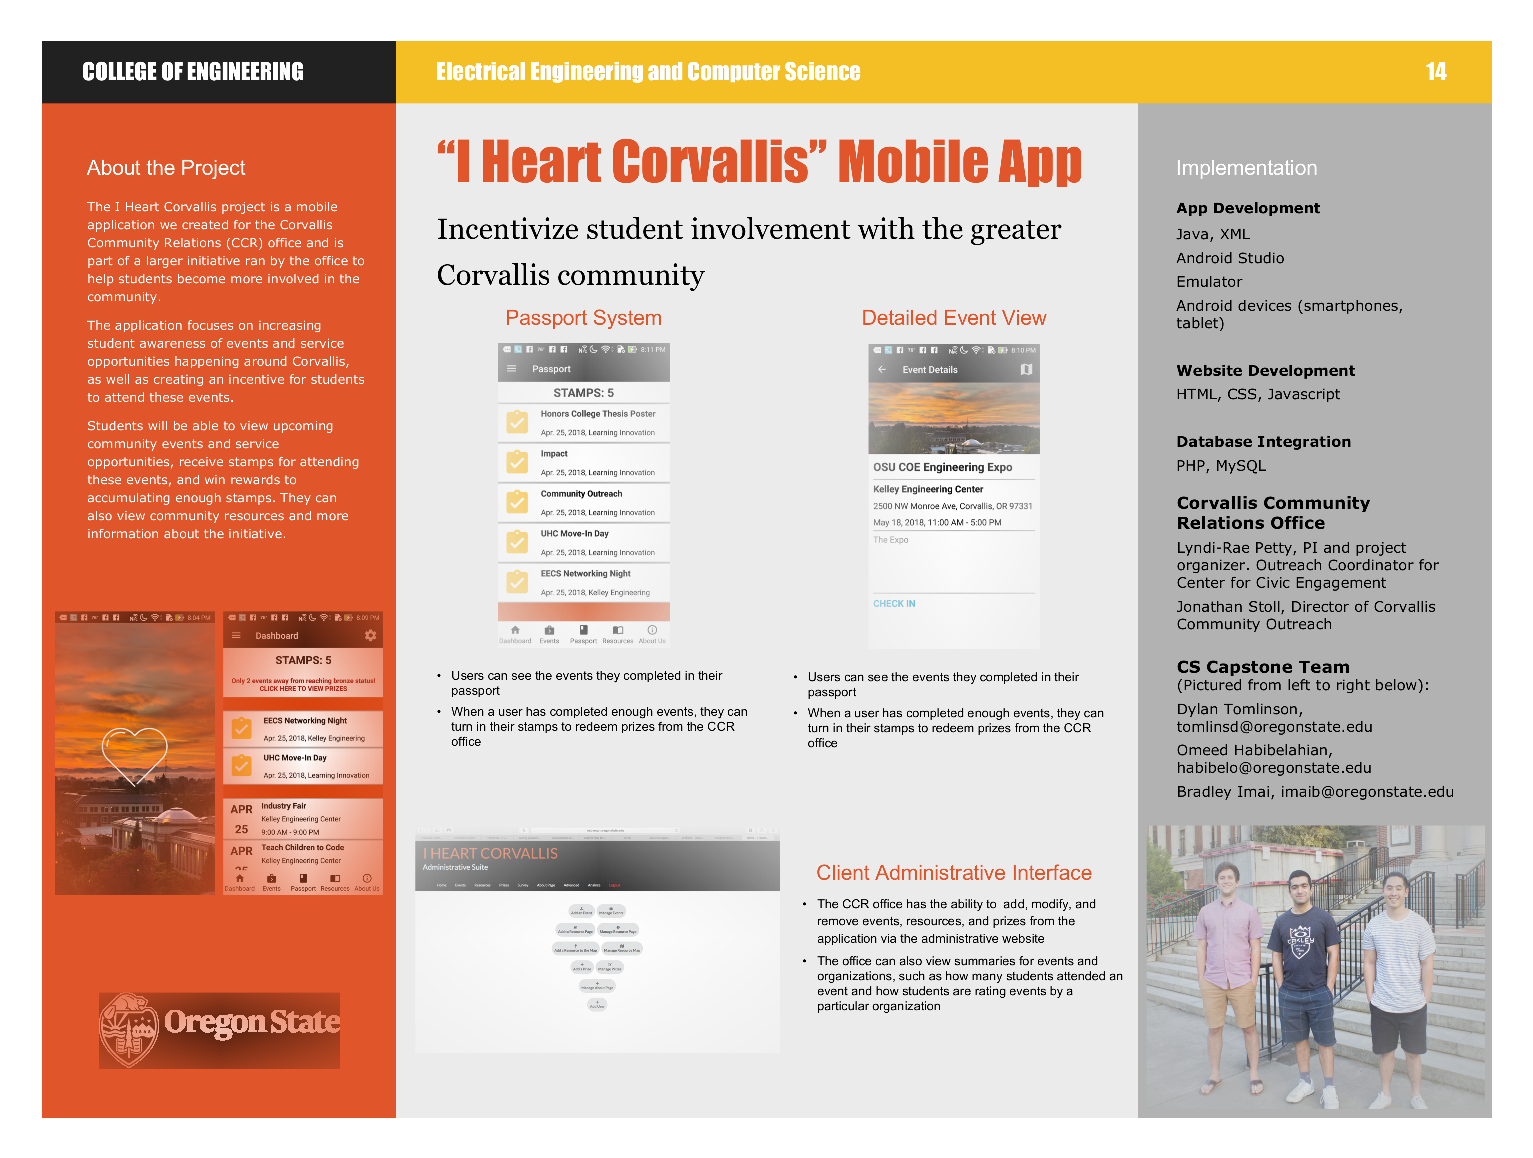
\includegraphics[height=13cm]{poster}
  \newpage

\section{Project Documentation}
  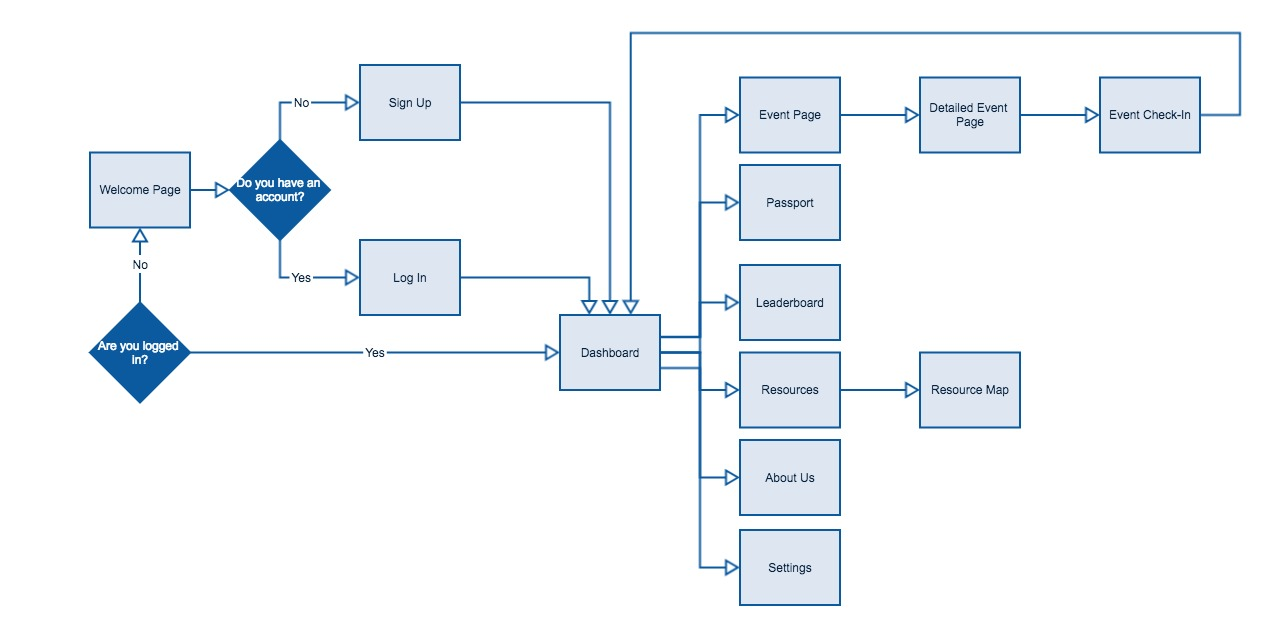
\includegraphics[height=8cm]{appflow} \\ \\
  \begin{center}
    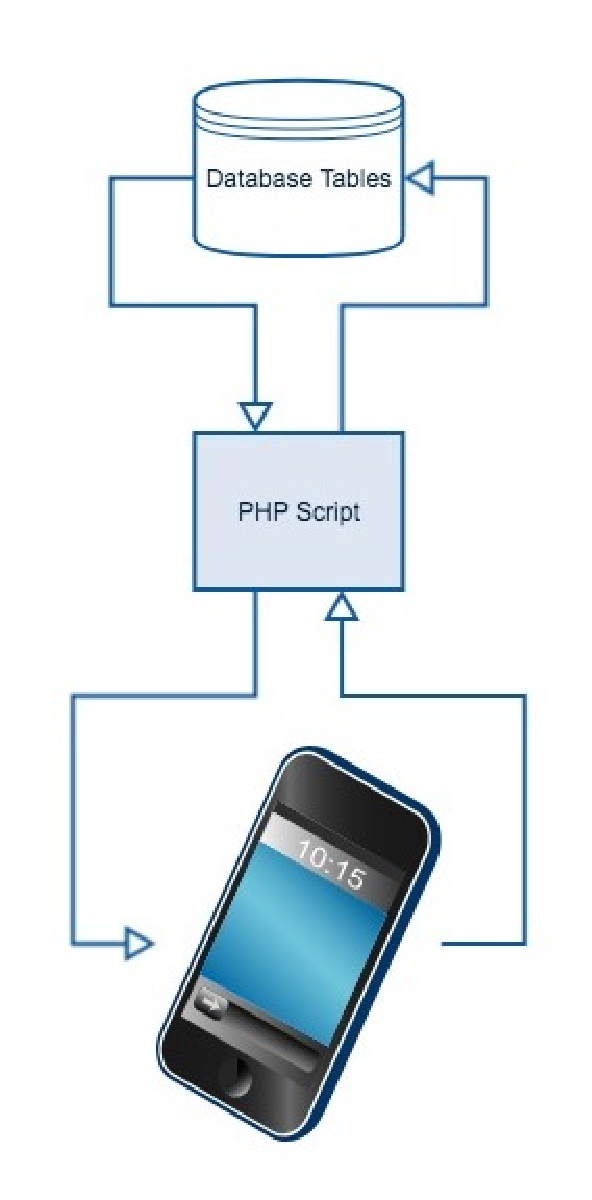
\includegraphics[height=8cm]{scriptflow}
  \end{center}
  The application provides users with a passport that shows them which events they have completed. Users receive stamps upon completing events, and when a user accumulates a sufficient number of stamps, they can redeem prizes. On the administrative website, the CCR office will be able to add, modify, and delete any content from the application, such as events, prizes, resources, resource map locations, survey questions, and the information displayed on the About Page. The office will also be able to authorize other users to access the administrative website. \\ \\
  The app has not yet been published to the Google Play Store, as the iOS version of the application has not yet been created. Once both versions of the application have been fully developed, the application will be published to both the Google Play Store and the Apple App Store. Once it is available on the Play Store, devices with Android 4.4 "KitKat" or later installed will be able to download the application from the Google Play Store. \\ \\
  In the meantime, in order to run the app, the device you want to run the app on must be connected to a computer that has both Android Studio installed and the full code directory for the app stored on it. To run the program in Android Studio, hit the Run button (the green Play button) at the top of the IDE and you will be able to choose whether you want the app to run on an emulator or on your own connected device. \\ \\

\section{Recommended Technical Resources to Learn More}
  \begin{itemize}
    \item Android Developers Website: \url{https://developer.android.com/}
    \item PBKDF2: \url{https://medium.com/@kasunpdh/how-to-store-passwords-securely-with-pbkdf2-204487f14e84}
    \item Derek Whiteside, Director of Web and Mobile Services at OSU
    \item Andrew Morgan, Systems Administrator, Identity and Access Management at OSU
  \end{itemize}
  \newpage

\section{Conclusions and Reflections}
  \subsection{Omeed}
    \subsubsection{What technical information did you learn?}
      I learned a lot about the visual design of applications, as well as how interactions between applications and databases are set up. It was really cool learning how each piece of the user interface visually comes together in the code. It took me a while to figure out exactly how applications connect to databases, and even though I would look through code tutorials, I continued to run into walls implementing it myself, but once I figured out an efficient implementation for one page, it was a lot easier to mold the code to fit for other pages of the app as well.

    \subsubsection{What non-technical information did you learn?}
      I learned a lot about how to communicate my creations to other people and how to modify my use of technical jargon to make my explanation as clear as possible to anyone who inquired about the project. This also applies to meeting with our client, as I had to effectively and clearly communicate our progress and next steps to our client, who did not have as much technical experience as us. I also learned how to schedule the completion of each task of a long-term endeavor, as the application and website had a slew of bits and pieces that we needed to make sure got completed in a timely manner.

    \subsubsection{What have you learned about project work?}
      I have learned that it’s important to communicate your progress and planned tasks to your teammates so there is no confusion as far as who is in charge of what tasks. I have also learned that dedicated teammates are crucial to completing everything that needs to get done for the project. This project has also taught me that plans change, and something that you thought would be a huge factor in the development of the project may end up being completely abandoned in the end. As you implement the project, your client may bring up new desires and change their mind on previous design decisions, and it is important to be aware of this when embarking on a time-intensive project.

    \subsubsection{What have you learned about project management?}
      As far as project management, this project taught me that it is incredibly important to plan out each task of the project and to set up a timeline for when to complete each task by. You also need to be clear when communicating your timeline to your teammates and client, as you need to ensure that not only your teammates are on board with your plan in relation to their plans, but also that your client agrees with your timeline. The final product is ultimately for the client, so they need to confirm that your schedule for completing each piece of the project aligns with their plans to deploy or market the final product. It is also very important to keep your progress saved in multiple places so that not only can you continue your work on different machines, but you have a backup of your data if you somehow lose your local files.

    \subsubsection{What have you learned about working in teams?}
      I have learned that each member of your team brings a different perspective to the table, whether it be for a particular piece of the project or for the project design as a whole. It is important to maintain your concept for the final product while simultaneously considering the concepts your teammates have created. They will undoubtedly have some idea for the project that you did not even think of, and the final product will reflect the decisions your team made on which features to implement and which ones to ignore or push to a later time. It is also very important to keep consistent contact with your team so you are not left in the dark about what the rest of your team is implementing.

    \subsubsection{\textbf{If you could do it all over, what would you do differently?}}
      If I were to do this project over again, I would definitely consider implementing the application with a cross-platform development environment. Our client's original goal was to have both an Android and iOS version of the application developed this year, and since we only had prior experience developing for iOS, we decided to focus on implementing the Android version of the application and making the iOS version a stretch goal. If I were to go back to Fall Term, I would do significantly more research on cross-platform development environments, such as React Native.

  \subsection{Bradley}
    \subsubsection{What technical information did you learn?}
      From the very beginning of the implementation stage of Winter term, every aspect of the programming and research was a new experience for me. My past experience in programming an Android application was the CS496 course at OSU.  We created a simple weather application that displayed weather data from an API. The I Heart Corvallis mobile application was an eye-opener for me in the Android development. Everything from the creation of an animated splash screen, utilizing Google Maps and displaying notable locations, geolocation, and implementing the ability for an Administration website to add, update and delete content that was displayed on the application was all a new experience for me.

    \subsubsection{What non-technical information did you learn?}
      Having the ability to talk nontechnical and technical in a working environment is essential to a successful project. In my past interviews for jobs, I have been asked every time to give an example of a nontechnical and technical experience. Over the course of this year, I had the ability to learn this skill and become proficient in it. Talking to our client whose background is nontechnical versus talking technical with group members was a slight barrier. However, I was able to pick up this skill easily and was able to successfully explain features and progress of our application to our client as well as discussing technical features of the application with group members.

    \subsubsection{What have you learned about project work?}
      This has been bar far the biggest project I have been a part of. Being able to organize and manage time in an efficient manner was a must in developing a successful application. Not only did I have to worry about completing my tasks for this application but I also had to worry about other coursework. The main factor that I took out of this coursework was that features took a lot longer than expected. Some of the smaller features of the application were able to develop in one setting but the majority of the features took at least a few days to program.

    \subsubsection{What have you learned about project management?}
      Reflecting this year, I noticed we took on a waterfall method for project management. This consisted of group members doing research, writing a requirement, design and technical documents in the fall, followed by implementation in the winter and bug fixing the spring. During the implementation phase, I noticed that we had to take a step back and modify our design and requirement decisions. This took us back a few days in which we could have been developing for our application. I have done some research on project management and many companies these days use the agile method. This consists of running through sprints and being able to develop a product in a more timely manner.

    \subsubsection{What have you learned about working in teams?}
      By working with an amazing group of guys, I was able to develop a specific set of experiences and skills that normal coursework could not. An example of this would be that groups make better decisions than individuals. Having multiple opinions of various features of the application gives ideas that may not have come up for an individual. Being able to work in a group environment is a must in the working field. No job, besides freelance will give you the option to work alone.

    \subsubsection{\textbf{If you could do it all over, what would you do differently?}}
      If I could do this all over again I would take a look at cross-platforming. After doing a few job search within mobile development I have seen a lot of React and React Native developers in need. From my understand React Native is a cross-platform framework that can develop for IOS and Android mobile application with use of javascript. Facebook developers had created this framework and have been widely used in Airbnb, Instagram, Discord and many more.

  \subsection{Dylan}
    \subsubsection{What technical information did you learn?}
      Basically every piece of code I wrote for this project was something new for me. I have only made one program using Java before, and it was extremely simple compared to this project. I also have never had experience working on a mobile application before. In terms of technical information I learned about the components that make up an android application. Such as having a Java class and XML layout for every page. I learned about how an android application uses resources and how to pass variables between classes. I also learned how to work with a hashing algorithm that is not part of a library. I also learned about how an android application communicates with a database. I always assumed that the PHP scripts would simply live with the application. I did not know that most applications simply use SQLite, storing information on the user’s phone instead of in a seperate database.

    \subsubsection{What non-technical information did you learn?}
      For non-technical info I learned how to set up and meet with actual computer scientists. We had a few situations throughout the year that required us to meet with employees of Oregon State. Through these meetings I feel that I learned a bit about the protocol of meeting with people in the field. I also learned about focus groups and getting user data. I had only been in one focus group and attended a few hosted by our client throughout the year. I also learned a bit about selling your work and having to describe it to technical and non technical people. Over the past month we have been trying to find a way for our project to live on after our graduation. We have met with the Visit Corvallis office and the marketing department of OSU in order to build up interest in our app. Nothing has come to fruition yet but it was still a good experience communicating our work and vision.

    \subsubsection{What have you learned about project work?}
      It helps to have others who are interested in working on the project. For my previous senior design project each of us split up the aspects of the project and none of us made much headway in the project. Having my group to work with through these requirements this year helped tremendously in keeping steady progress throughout the year. We have been able to keep each other accountable and motivated to work on the application. I have also learned that it takes a lot of time, between getting approval from our client and the actual time it takes to code in a feature, a lot of time passes. Most of these requirements took several days if not weeks to complete. When creating something new you generally can’t expect to sit down and finish it in one sitting.

    \subsubsection{What have you learned about project management?}
      I have learned the importance of planning for the worst. Leaving extra time later in the development cycle is the main reason why we were able to complete this project. We began development during winter break as we knew this project was going to take a lot of planning. That planning paid out by allowing us to work when we had time instead of having to cram our schedules half way through the term. There were very few times that I was worried about the project as we were generally ahead of where we needed to be in the development cycle.

    \subsubsection{What have you learned about working in teams?}
      Communication has been the most important factor in working as a team. We have several different outlets for communicating that we have been using frequently throughout the year. Finding times to work together was always a challenge but we managed, spending many late nights at the Valley Library over winter term. It is also important to communicate your work to your teammates. If you are having a specific problem, they could usually offer some sort of insight to help out.

    \subsubsection{\textbf{If you could do it all over, what would you do differently?}}
      I would have started the CAS implementation earlier in the development cycle. We did not realize that it would be much more difficult to implement CAS in a mobile application than in a website. If we had started it in the winter, than we might have been able to finish it. I also would have looked further into cross platform development. We did a lot of research on the subject, but we had our worries that it wouldn’t work out well. It would have been great to have an iOS and an Android version of our app.

  \newpage

\section{Appendix I: Essential Code Listings}
  \subsection{EventListAdapter Class}
    \begin{lstlisting}[style=java]
package edu.oregonstate.studentlife.ihcv2.adapters;

import android.support.v7.widget.RecyclerView;
import android.util.Log;
import android.view.LayoutInflater;
import android.view.View;
import android.view.ViewGroup;
import android.widget.LinearLayout;
import android.widget.TextView;

import java.util.ArrayList;
import java.util.Date;

import edu.oregonstate.studentlife.ihcv2.R;
import edu.oregonstate.studentlife.ihcv2.data.Event;

/**
* Created by Omeed on 1/18/18.
*/

public class EventListAdapter extends RecyclerView.Adapter<EventListAdapter.EventListViewHolder> {

private ArrayList<Event> mEventList;
private OnEventClickListener mOnEventClickListener;
private final static String TAG = EventListAdapter.class.getSimpleName();

public EventListAdapter(OnEventClickListener onEventClickListener) {
  mEventList = new ArrayList<Event>();
  mOnEventClickListener = onEventClickListener;
}

public void addEvent(Event event) {
  mEventList.add(event);
  notifyDataSetChanged();
}

@Override
public int getItemCount() {
  return mEventList.size();
}

public interface OnEventClickListener {
  void onEventClick(Event event);
}

@Override
public EventListViewHolder onCreateViewHolder(ViewGroup viewGroup, int viewType) {
  LayoutInflater inflater = LayoutInflater.from(viewGroup.getContext());
  View view = inflater.inflate(R.layout.event_item_listview, viewGroup, false);
  EventListViewHolder viewHolder = new EventListViewHolder(view);
  return viewHolder;
}

@Override
public void onBindViewHolder(EventListViewHolder holder, int position) {
  Event event = mEventList.get(position);
  holder.bind(event);
}

class EventListViewHolder extends RecyclerView.ViewHolder {

  private LinearLayout mEventListingLL;
  private TextView mEventMonthTV;
  private TextView mEventDayTV;
  private TextView mEventNameTV;
  private TextView mEventLocationTV;
  private TextView mEventTimeTV;

  private String[] monthShortNames = {"JAN", "FEB", "MAR", "APR", "MAY", "JUN", "JUL", "AUG", "SEP", "OCT", "NOV", "DEC"};

  public EventListViewHolder(View itemView) {
    super(itemView);
    mEventListingLL = (LinearLayout) itemView.findViewById(R.id.ll_event_listing);
    mEventMonthTV = (TextView) itemView.findViewById(R.id.tv_event_month);
    mEventDayTV = (TextView) itemView.findViewById(R.id.tv_event_day);
    mEventNameTV = (TextView) itemView.findViewById(R.id.tv_event_name);
    mEventLocationTV = (TextView) itemView.findViewById(R.id.tv_event_location);
    mEventTimeTV = (TextView) itemView.findViewById(R.id.tv_event_time);

    mEventListingLL.setOnClickListener(new View.OnClickListener() {
      @Override
      public void onClick(View v) {
        mOnEventClickListener.onEventClick(mEventList.get(getAdapterPosition()));
      }
      });
    }

    void bind(Event event) {
      mEventNameTV.setText(event.getName());
      mEventLocationTV.setText(event.getLocation());
      Log.d(TAG, "start dt: " + event.getStartDay() + "-" + event.getStartMonth() + "-" + event.getStartYear() + " " + event.getStartTime());
      Log.d(TAG, "end dt: " + event.getEndDay() + "-" + event.getEndMonth() + "-" + event.getEndYear() + " " + event.getEndTime());
      if (event.getStartDay().equals("1") &&      event.getStartMonth().equals("1") && event.getStartYear().equals("1900") && event.getStartTime().equals("12:00 AM")
      && event.getEndDay().equals("31") && event.getEndMonth().equals("12") && event.getEndYear().equals("2099") && event.getEndTime().equals("11:59 PM")) {
        mEventMonthTV.setText("ANY");
        mEventDayTV.setText("TIME");
        mEventTimeTV.setText("Anytime");
      }
      else {
        int monthInt = Integer.parseInt(event.getStartMonth()) - 1;
        mEventMonthTV.setText(monthShortNames[monthInt]);
        mEventDayTV.setText(event.getStartDay());
        String dtRange = event.getStartTime() + " - " + event.getEndTime();
        mEventTimeTV.setText(dtRange);
      }
    }

  }

}

    \end{lstlisting}
    \newpage

  \subsection{PassportLoader Class}
    \begin{lstlisting}[style=java]
package edu.oregonstate.studentlife.ihcv2.loaders;

import android.content.Context;
import android.support.v4.content.AsyncTaskLoader;
import android.util.Log;

import java.io.BufferedReader;
import java.io.InputStreamReader;
import java.io.OutputStreamWriter;
import java.net.HttpURLConnection;
import java.net.URL;
import java.net.URLEncoder;

/**
 * Created by Omeed on 2/22/18.
 */

public class PassportLoader extends AsyncTaskLoader<String> {
    private final static String TAG = PassportLoader.class.getSimpleName();

    private String userid;
    private String passportJSON;
    private final static String IHC_GET_COMPLETED_EVENTS_URL = "http://web.engr.oregonstate.edu/~habibelo/ihc_server/appscripts/get_completed_events.php";

    public PassportLoader(Context context, String userid) {
        super(context);
        this.userid = userid;
    }

    @Override
    protected void onStartLoading() {
        forceLoad();
    }

    @Override
    public String loadInBackground() {
        try {
            URL url = new URL(IHC_GET_COMPLETED_EVENTS_URL);
            String data = URLEncoder.encode("userid", "UTF-8") + "=" + URLEncoder.encode(userid, "UTF-8");

            HttpURLConnection conn = (HttpURLConnection) url.openConnection();

            conn.setRequestMethod("POST");
            conn.setDoOutput(true);
            OutputStreamWriter wr = new OutputStreamWriter(conn.getOutputStream());
            wr.write( data );
            wr.flush();

            BufferedReader reader = new BufferedReader(new InputStreamReader(conn.getInputStream()));

            StringBuffer sb = new StringBuffer("");
            String line = null;

            while ((line = reader.readLine()) != null) {
                sb.append(line);
            }

            return sb.toString();
        } catch (Exception e) { e.printStackTrace(); return new String("Exception: " + e.getMessage()); }
    }

    @Override
    public void deliverResult(String data) {
        passportJSON = data;
        Log.d(TAG, "passport data: " + data);
        super.deliverResult(data);
    }

}
    \end{lstlisting}
    \newpage

  \subsection{Recording a Completed Event}
    \begin{lstlisting}[style=php]
<?php

ini_set('display_errors', 1);
error_reporting(E_ERROR);
ini_set('memory_limit', '1G');

$dbhost="oniddb.cws.oregonstate.edu";
$dbname="habibelo-db";
$dbuser="habibelo-db";
$dbpass="RcAbWdWDkpj7XNTL";

$alreadyExists = False;

$mysqli = new mysqli($dbhost,$dbuser,$dbpass,$dbname);
//Output any connection error
if ($mysqli->connect_error) {
  die('Error : ('. $mysqli->connect_errno .') '. $mysqli->connect_error);
}

$userid = $eventid = "";

if ($_SERVER["REQUEST_METHOD"] == "POST") {
  $userid = $_POST["userid"];
  $eventid = $_POST["eventid"];
  $rating = $_POST["rating"];
  $comment = $_POST["comment"];
  $dateandtime = date("Y-m-d H:i:s");

  $stmt = $mysqli->prepare("INSERT INTO ihc_completed_events (userid, eventid, dateandtime, rating, comment) VALUES (?, ?, ?, ?, ?)");
  $stmt->bind_param('iisis', $userid, $eventid, $dateandtime, $rating, $comment);
  $stmt->execute();
  if ($stmt->get_error == "") {
    $stmt2 = $mysqli->prepare("SELECT * FROM ihc_completed_events WHERE userid=?");
    $stmt2->bind_param('i', $userid);
    $stmt2->execute();
    if ($stmt2->error == "") {
      $result = $stmt2->get_result();
      $stampcount = $result->num_rows;

      $stmt3 = $mysqli->prepare("UPDATE ihc_users SET stampcount=? WHERE id=?");
      $stmt3->bind_param('ii', $stampcount, $userid);
      $stmt3->execute();
      if ($stmt3->error == "") {
        echo "COMPLETED EVENT ADDED";
      }
      $stmt3->close();
    }
    $stmt2->close();
  }
  else {
    echo "ADDERROR";
  }
  $stmt->close();
}

$mysqli->close();
?>
    \end{lstlisting}
    \newpage

  \subsection{Updating a Prize}
    \begin{lstlisting}[style=php]
<?php

ini_set('display_errors', 1);
error_reporting(E_ERROR);
ini_set('memory_limit', '1G');

$dbhost="oniddb.cws.oregonstate.edu";
$dbname="habibelo-db";
$dbuser="habibelo-db";
$dbpass="RcAbWdWDkpj7XNTL";

$alreadyExists = False;

$mysqli = new mysqli($dbhost,$dbuser,$dbpass,$dbname);
//Output any connection error
if ($mysqli->connect_error) {
  die('Error : ('. $mysqli->connect_errno .') '. $mysqli->connect_error);
  echo "Connection failed!<br>";
}

$prizeid = $name = $level = "";

if ($_SERVER["REQUEST_METHOD"] == "POST") {
  $prizeid = $_POST["prizeid"];
  $name = $_POST["name"];
  $levelVal = $_POST["level"];

  if ($levelVal == "1") {
    $level = "gold";
  }
  else if ($levelVal == "2") {
    $level = "silver";
  }
  else if ($levelVal == "3") {
    $level = "bronze";
  }

  $stmt = $mysqli->prepare("UPDATE ihc_prizes SET name=?, level=? WHERE prizeid=?");
  $stmt->bind_param('ssi', $name, $level, $prizeid);
  $stmt->execute();

  if ($stmt->error == "") {
    $message = "Prize has been updated!";
  }
  else {
    $message = "Error updating prize!"; # error updating prize in database
  }
  $url = "../manage_prizes.php";

  $stmt->close();
  $mysqli->close();
  echo "<script type='text/javascript'>alert('$message');</script>";
  echo "<script type='text/javascript'>document.location.href = '$url';</script>";
}
$mysqli->close();

?>
    \end{lstlisting}
  \newpage

\section{Appendix II: Screenshots}
  \subsection{Application}
    \includegraphics[height=8cm]{splash}
    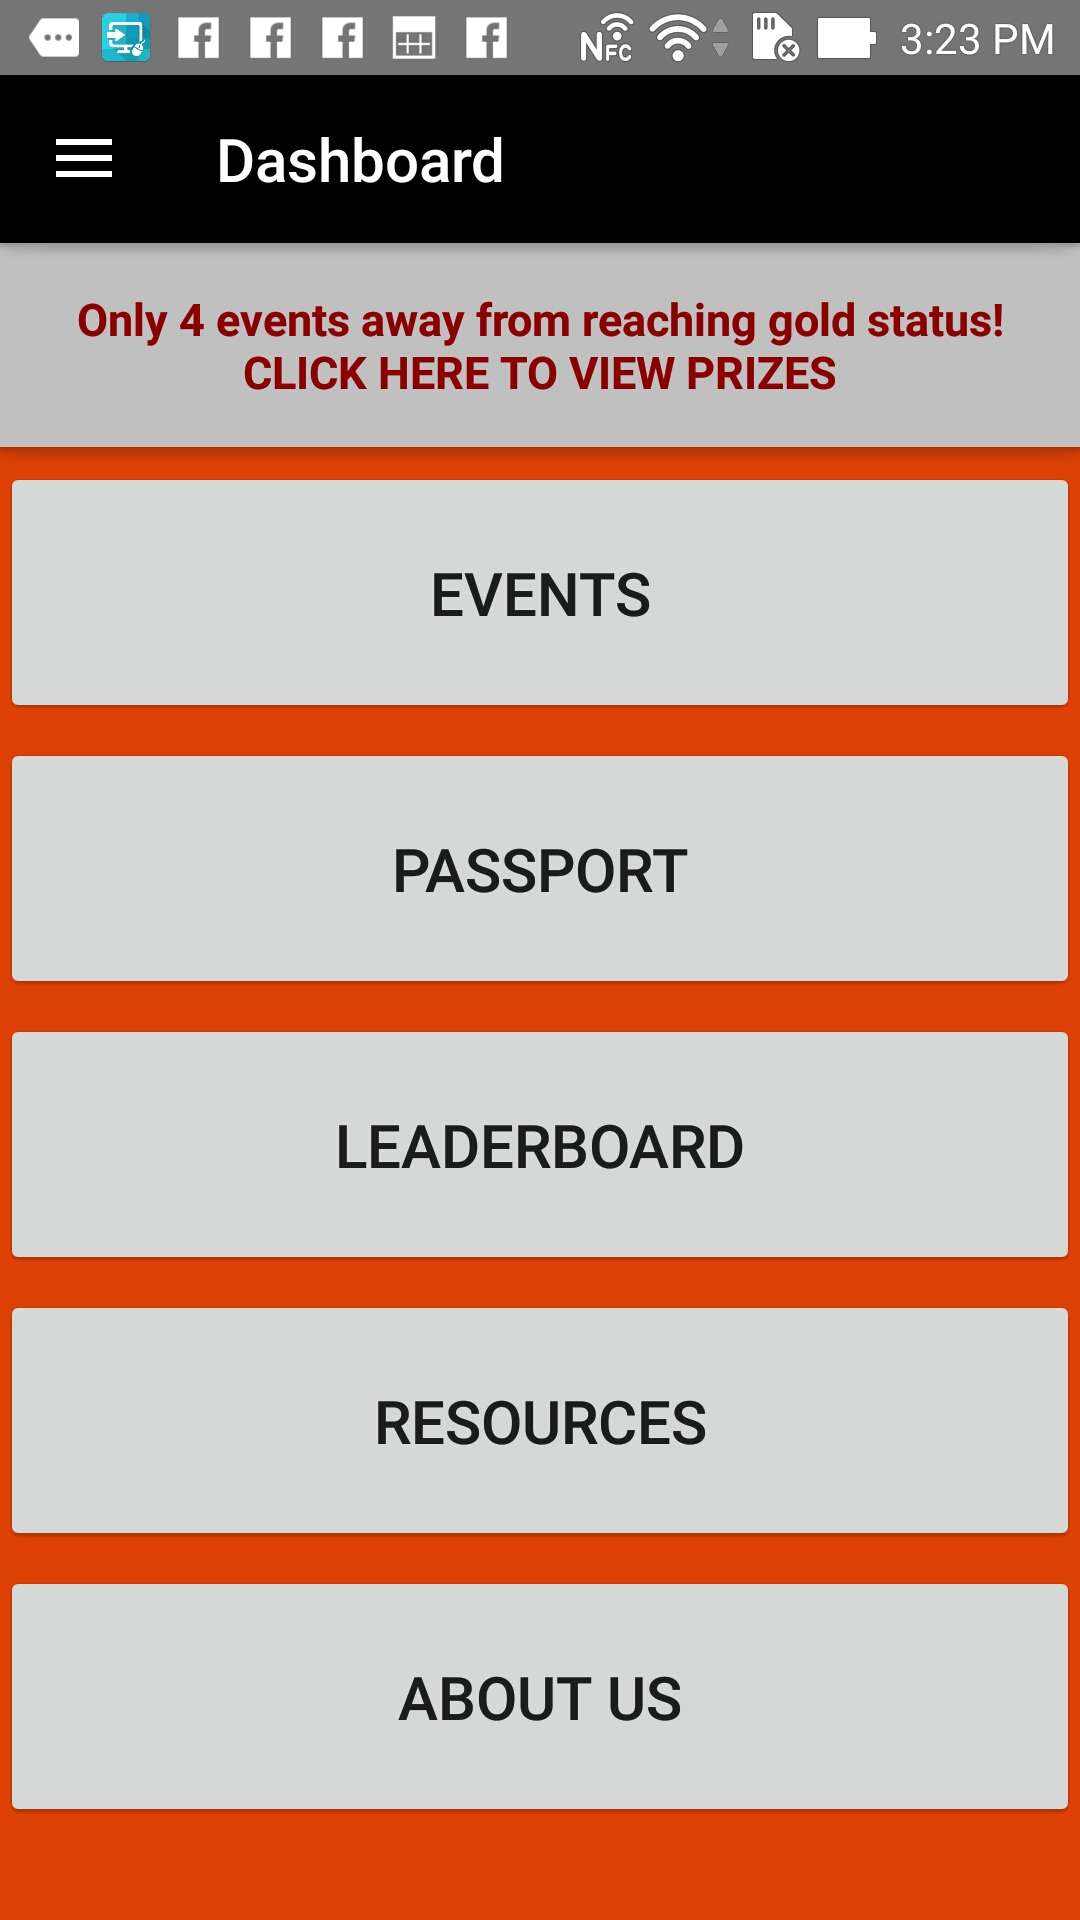
\includegraphics[height=8cm]{dashboard}
    \includegraphics[height=8cm]{eventdetail}
    
\includegraphics[height=8cm]{passport}
    \includegraphics[height=8cm]{eventmap}
    \includegraphics[height=7cm]{website} \\
    Top left: Splash screen \\
    Top second from left: Dashboard \\
    Top second from right: Event Detail Page \\
    Top right: Passport \\
    Bottom left: Event Map \\
    Bottom right: Administrative Website Homepage \\

\end{document}
